\documentclass{standalone}
\usepackage{tikz}

%: === TIPOGRAFÍA === (((
\usepackage{fontspec}
\setmainfont[
  BoldFont       = bodonibi,
	ItalicFont     = Century modern italic2.ttf,
	BoldItalicFont = bodonibi,
	SmallCapsFont  = lmromancaps10-regular.otf
]{Century_modern.ttf}
\DeclareSymbolFont{italics}{\encodingdefault}{\rmdefault}{m}{it}
\DeclareSymbolFontAlphabet{\mathit}{italics}
\ExplSyntaxOn
\int_step_inline:nnnn { `A } { 1 } { `Z }
 {  \exp_args:Nf \DeclareMathSymbol{\char_generate:nn{#1}{11}}{\mathalpha}{italics}{#1} }
\int_step_inline:nnnn { `a } { 1 } { `z } {  \exp_args:Nf \DeclareMathSymbol{\char_generate:nn{#1}{11}}{\mathalpha}{italics}{#1}}
\ExplSyntaxOff
% )))

\begin{document}

\begin{tikzpicture}[>=latex]
	\clip (-4,0) rectangle (6.5,4);
	% \fill [gray!20] (0,0) rectangle (-4cm,4cm);
	\draw (0,0) rectangle (-4,4);
	\node at (-2,2) {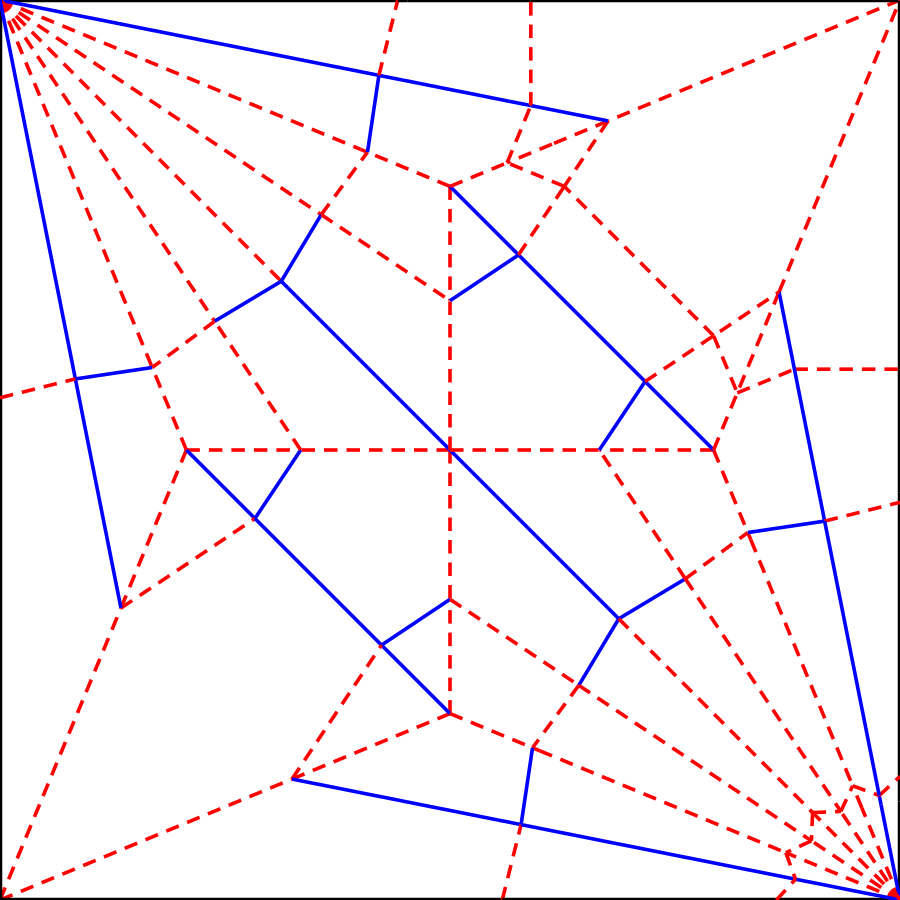
\includegraphics[width = 4cm, height = 4cm]{crane.png}};
	\node at (4.5,2) {
\includegraphics[width = 4cm, height = 4cm]{swan.png}};
	\draw [->, xshift=0.4cm] (0.2,2) to [out=20 , in=160] node [above,midway] {\(T\)} (1.8,2);
\end{tikzpicture}

\end{document}
